\documentclass[12pt,a4paper]{article}
\usepackage{authblk}
\usepackage{float}
\usepackage[margin=1in]{geometry}
\usepackage{fancyhdr}
\usepackage{hyperref}
\usepackage{graphicx}
\usepackage{babel}
\usepackage{csquotes}

\usepackage[toc,page]{appendix}
\usepackage{makecell}
\newcommand{\tabitem}{\\~~\llap{\textbullet}~~}

\pagestyle{fancy}

\title{GPT Pedagogy}
\author[1]{Matthew Pisano\quad\href{mailto:pisanm2@rpi.edu}{pisanm2@rpi.edu}}
\author[1]{\\Tiburon Benavides\quad\href{mailto:benavt@rpi.edu}{benavt@rpi.edu}}
\author[1]{\\Lu Zhou\quad\href{mailto:zhoul12@rpi.edu}{zhoul12@rpi.edu}}
\author[1]{\\Yanshen Lin\quad\href{mailto:liny16@rpi.edu}{liny16@rpi.edu}}
\author[1]{\\Yiyang Cai\quad\href{mailto:caiy3@rpi.edu}{caiy3@rpi.edu}}
\affil[1]{Rensselaer Polytechnic Institute}
\date{\today}

\begin{document}
    \maketitle

    \abstract{
        GPT-3 and related technologies, while transformative, can be misused by students, hindering
        their learning potential. This paper presents a technical use case description for a GPT-3-based
        tool designed to foster transparency, active learning, and engagement between instructors and
        students in higher education. Our objective in designing this tool aligns with the fourth UN SDG,

        \begin{quote}
            Ensure inclusive and equitable quality education and promote lifelong
            learning opportunities for all~\cite{sdg}.
        \end{quote}

        We propose an asynchronous and adaptive learning tool that supports, rather than undermines,
        the educational process.

        Our learning assistant, named \textit{Mathesis} from the ancient greek work for learning,
        will be integrated in an Introduction to Biology course at RPI during the Fall 2023 semester.
        In collaboration with institute faculty members, we have gathered ample course material to
        fine-tune a GPT-3~\cite{gpt3} model. When integrated with our online user interface, this model can be
        used by students as a domain-knowledgeable and adaptive learning assistant. This personalized
        AI tutor aims to facilitate learning, increase transparency, and reduce student stress.

        Our goal for \textit{Mathesis} is to retain the conversational abilities of ChatGPT while
        fine-tuning the underlying large language model (LLM) with domain expertise. The current
        fine-tuned model can perform several tasks that achieve this goal.  These include: the generation
        of course-relevant multiple choice and free response questions, the assessment of student
        responses, and the generation of tailored, critical, and constructive feedback to students.
        Future model iterations will leverage human-in-the-loop reinforcement learning, drawing from
        previous interactions with students and faculty to expand its proficiency as a learning tool.

        We also aim for this model to be generalizable to other classes and disciplines in the future.
        The model will work especially well for courses where it is difficult to give personalized
        feedback to each learner in each class meeting time. This often happens in classes that have
        a high student to faculty ratio.
    }

    \pagebreak

    \section{Introduction}

    Large language models (LLMs), such as OpenAI's Generative Pre-trained Transformer (GPT) series,
    have revolutionized the field of natural language processing (NLP) with their advanced language
    understanding and generation capabilities. These models are based on deep learning architectures
    called transformers, which enable the efficient processing of vast amounts of textual data. LLMs
    are trained on extensive datasets containing diverse information from websites, books, articles,
    and other sources, allowing them to grasp context and generate human-like responses. GPT-3, one of
    the latest iteration in the series, has shown remarkable performance in various tasks, including
    translation, summarization, and question-answering. While these models hold immense potential
    for applications across different domains, their use in educational settings has gained significant
    attention. By leveraging the proficiency of LLMs like GPT-3, we aim to develop an innovative
    learning tool that enhances student engagement and promotes a more personalized learning experience.

    \subsection{Our Targeted Approach}

    In partnership with the Teaching and Learning Collaboratory (TLC) at Rensselaer Polytechnic
    Institute (RPI) in Troy, NY, we have identified an Introduction to Biology class section in the
    Fall 2023 semester for the debut of our GPT-based learning management system. We believe \textit{Mathesis}
    will significantly benefit students by providing them with relevant questions and detailed
    knowledge of course topics. This targeted approach reduces uncertainty and increases the model's
    usefulness to students by generating responses specific to the course material, avoiding
    misinformation or demotivation.

    \subsection{Significance}

    Customized learning assistants like \textit{Mathesis} have the potential to reshape the educational
    landscape. We do not contend that AI models can replace faculty, rather that they can serve as
    learning aids to students. In this role, the model continuously assesses and reinforces 
    student competency in course-relevant material by answering questions and providing feedback on
    self-administered assessments.  The potential impact of these assistants is especially significant
    in courses with an elevated student-to-faculty ratio.  In these classes, each student is 
    afforded a limited amount of personalized instruction from the professor or their TAs. Automated
    learning assistants can provide students another avenue of learning from a domain-knowledgeable entity.
    This paradigm has the additional benefit of allowing faculty to prioritize their personalized
    instruction time on particular students in need of assistance beyond the capabilities of an automated
    assistant.  Similar initiatives, such as Khan Academy's Khanmigo~\cite{khanmigo}
    model, offer comparable services to K-12 education through their online educational platform.
    We hypothesize that integration of LLM tutors in higher education will result in an elevated
    level of conceptualization of course material among affected students.

    \let\thefootnote\relax\footnotetext{Our source code can be found at:
    \href{https://github.com/ITWSXInformatics/ChatGPT_Pedagogy_Group2_2023}{\textit{github.com/ITWSXInformatics/ChatGPT\_Pedagogy\_Group2\_2023}}}

    \let\thefootnote\relax\footnotetext{A demo video can be found at:
    \href{https://drive.google.com/file/d/139m_XDbhoRpS4L9yhUWEu-zSxkCSfSdE/view?resourcekey}{\textit{drive.google.com/file/d/139m\_XDbhoRpS4L9yhUWEu-zSxkCSfSdE}}}

    \section{Project Use Case}

    \subsection{Specifications}

    For the development of the use case for this project, it is important to detail several
    specifications that describe GPT Pedagogy in a more rigorous manner.  One of these specifications
    is the list of the requirements of the project.  To fulfil our objectives, the
    project has the following \textit{functional requirements}:

    \begin{itemize}
        \label{functionalReqs}

        \item Be able to confidently and correctly answer any course-relevant question
        \item Be able to generate questions for students, based on key learning objectives
        \item Receive and evaluate student answers
        \item Provide useful feedback to students on their answers
        \item Allow instructors to customize question generation
        \item Allow instructors to evaluate class performance on key learning objectives
    \end{itemize}

    Along with these functional requirements, the project requires several \textit{non-functional
    requirements}.  Our project must also have:

    \begin{itemize}
        \label{nonFunctionalReqs}
        \item A GPT model fine-tuned to course-relevant material
        \item A user interface students and administrators use to interact with the model
        \item A login and authentication system to prevent unwanted access and to keep track of evaluations
    \end{itemize}

    Another important specification to consider is that of the entropy/uncertainty of the project.
    Overall, we have worked to minimize the total uncertainty of the project.  It is important to note,
    however, that the GPT model will always introduce some amount of extra uncertainty.

    One of the areas where we worked to minimize uncertainty is through the fine-tuning of the model on our
    own, customized, training data. The use of a GPT model introduces some uncertainty in user experience.
    However, we have minimized uncertainty associated with use of the model by employing fine-tuning
    and prompt engineering techniques. Fine-tuning enables confidence in our model's ability to provide
    accurate information on course-related concepts. Whereas prompt engineering tailors model outputs
    to fit within designed specifications which are amenable to integration within our user interface.

    We also minimized uncertainty by careful user interface design.  Our UI has
     two views corresponding to the student and administrator users.  In both of these cases, our design
    was oriented towards a simple, straightforward interface.  We worked to accomplish this through
    the use of a minimalist design.  Users can choose to choose only a few tabs: the main chat and
    the lesson evaluations.  The administrators have a similar view, with the addition of the ability
    to edit the questions that are displayed to students.  In our design buttons, animations, and
    images are kept to a minimum.  This allows users to focus key features of the website including 
    evaluations or interactions with \textit{Mathesis}.

    The use case that we developed addresses what we expect to be the basic flow of the system, along
    with any reasonable alternate or exception flows.  The goal of this system is the same as the
    project in general: to use an interface and pre-trained model to provide students with a flexible
    and helpful learning assistant for the \textit{Introduction to Biology} course at RPI.

    We have included the particular flows that we did in order to properly scope our use case.  Our intention
    is to implement all relevant ways in which students and administrators interact with the system,
    while not including flows that may bloat our design of this early use case.  Examples
    of such flows would be deliberate adversarial attacks to the system.  While these attacks are a
    near certainty in a deployed system, the time constraints on this project has not allowed us to
    account for them in our working prototype. Due to this reason, we have set this, and similar
    edge cases, to be outside our implementation scope.

    \subsection{Semiotic Implementation Considerations}

    As mentioned above, one of our primary design goals of this project was to minimize uncertainty.
    In addition to the previously mentioned methods, we also minimized uncertainty through our
    usage of semiotics, cognitive principles, and the project architecture.

    One of the ways in which we minimize uncertainty is through our placement of our signs.  Many
    of the elements in the user interface lack symbols or icons.  This is by design.  As this project
    is currently in a prototype form, it would be unwise to begin using signs in places where they do
    not need to be.  In place of these signs we instead have text descriptions.  While this may be
    less visually appealing, it offers a lower uncertainty as many elements have their descriptions
    written on them.  An example of a sign that we \textit{do} use can be found in the 'send' icon for the
    chat functionality.  This sign is an icon, specifically, as it does not physically resemble anything
    being sent.  We chose this icon to be that of a paper airplane, as is standard across most
    massaging applications.  Through the use of this, and other icons, we hope to make all functionality
    clear while maintaining familiarity.  Another icon that we use in our interface is the \textit{Mathesis}
    logo.  This sign is also an icon, as it does not attempt to capture the appearance of our learning
    assistant, even if there was one.  It is designed with a similarly minimalist style.  Our goal with
    this sign is to give students something unique to associate with the project.  Through this
    association, we hope that students will be more engaged with our site as it has a unique color
    palette, design, and character.

    We also use both semiotics and cognitive principles in the chat and feedback functionalities of
    the project.  Our design of the chat and feedback interfaces mirrors that of more mundane chat-focused
    applications.  By modeling our interface in a similar manner to SMS communications, we create a
    familiar environment to both students and teachers.  This was likely the rationale of ChatGPT's
    interface design, which mirrors these communications as well.  The 'lesson quiz submission' view also
    mirrors other systems, such as RPI's learning management systems (LMS).  In general, we create an
    environment that borrows many of the qualities that are present in other applications that are
    familiar to students. By using this familiarity, we hope that users will be able to immediately
    recognize the form and function of the interface, allowing for quicker acclimation.

    \subsection{Alignment and Feedback Considerations}

    Several considerations are specific to early adoption in the Introduction to Biology course at RPI.
    This course deals with several topics which could be scrutinized by students with disparate
    experiences, beliefs, and upbringings including: human evolution, origins of Earth, Covid-19,
    and climate change. While it is most likely impossible to robustly account for each of the various
    views on each topic, we have already made significant strides to fine-tune the underlying model
    to respect student’s views while also making them aware of the current prevailing consensus in
    the biological literature. \textit{Mathesis'} role is to educate, not to indoctrinate. For this reason,
    our model's behavior towards student's stated beliefs is trained to be both respectful and
    agnostic of doctrine. In the future, a topic blacklist may be curated to prevent students from
    asking the learning assistant questions misaligned with course concepts. Topics on this blacklist
    may involve disparate conspiracy theories prevalent in modern online discourse. When a question
    regarding one of these topics is asked, the response will be hard-coded to redirect the student's
    question to the human faculty member.

    Our system is designed to be customizable and scalable to fit future needs of higher education.
    While we have partnered with a professor in the Biology department, there are other courses at
    RPI which may benefit from a personalized AI tutor like \textit{Mathesis}. Our platform is
    designed to be amenable to a broad spectrum of course curricula. Each course at RPI can be
    subdivided into units, and each unit can be further divided into key learning objectives. The
    fine-tuned models are trained to be proficient question-answering systems per each stated key
    learning objective. Furthermore, significant supplemental documentation of the fine-tuning
    process will be made available for domain-knowledgeable models to be created for other courses.
    For some courses like calculus and physics, it may be necessary to incorporate more updated
    models, like GPT-4, which have image + text modality~\cite{openAiDocs,gpt4}. This modality would
    enable students to upload images of their work to be assessed by the system.

    Finally, our system will employ a student and faculty feedback component to allow continuous
    improvement of the resource. This ability will allow users to report issues or flag model outputs,
    suggest improvements, and contribute to the model's ongoing refinement. By providing users a
    voice in the future development of this project, we hope to make the \textit{Mathesis} learning assistant
    more inclusive, accommodating, and adaptable to a wide range of student and faculty interactions.

    \section{Architectural Models}

    \subsection{Conceptual Model}
    
    In our conceptual model, we outline the general structure of our project, its core components,
    and how those components relate to each other.

    \begin{figure}[H]
        \centering
        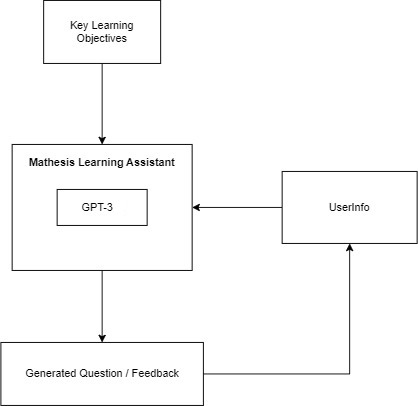
\includegraphics[width=0.8\textwidth]{images/conceptualDiagram}
        \caption{Conceptual Model}
        \label{fig:conceptualModel}
    \end{figure}
    

    \paragraph{Mathesis}
    The core of our project is our \textit{Mathesis}
    learning assistant, powered by GPT-3.  This is placed at the center of the diagram, symbolizing
    its foundational role. It is important to include this component in our diagram as it is the main
    generator of content for the project.  This content can be anything from novel quiz questions to
    feedback for students. In our diagram, \textit{Mathesis} is shown as a wrapper with a core of
    GPT-3.  This is because our implementation is an extension and customization of OpenAI's model, created
    to achieve the project's specific goals. In our case, the base model provides the core language
    understanding and generation capabilities that the \textit{Mathesis} Learning Assistant builds
    upon with its own knowledge and understanding.

    \paragraph{Key Learning Objectives}
    Also in our model, we include key learning objectives as an object.  This object represents the
    collection of core course material that students are meant to learn.  It is connected to our model,
    highlighting their guiding role in shaping the model's behavior through fine-tuning. These
    objectives ensure that the model focuses on the most important topics and concepts as defined by
    the faculty. The assistant generates questions and provides feedback on student's performance
    based on these key learning objectives.

    \paragraph{Model Output}
    In our diagram, we also include the products of the learning assistant.  This is important to include
    because it shows what the model actually does to deserve its role as central to the function of
    the project.  This output comes in the form of questions, generated from the learning objectives
    of the course, and useful feedback and corrections to the answers of students.  This feedback also
    encapsulates the chat functionality of the model, where it provides feedback based on any question
    that the user asks of it.

    \paragraph{User Information System}
    Finally, the UserInfo MongoDB Database stores user information and their corresponding performance
    data for specific chapters.  This will be useful to help gauge the quality of the questions that
    the model produces and the areas that the students may be struggling the most in.  Both scenarios
    help to guide faculty into improving the course in some way.

    
    \subsection{Logical Model}
    
    Our logical model both maintains the objects and relations of the conceptual model and builds upon
    them through extra details about attributes and typing.

    \begin{figure}[H]
        \centering
        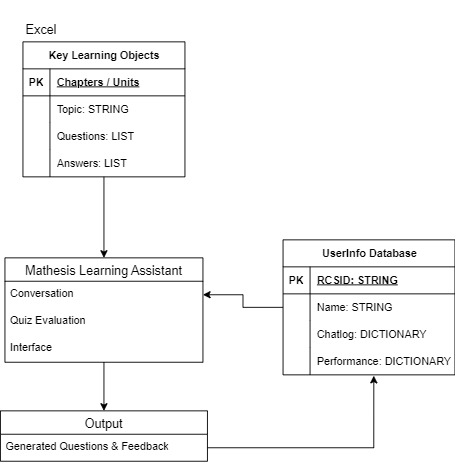
\includegraphics[width=0.8\textwidth]{images/logicalDiagram}
        \caption{Logical Model}
        \label{fig:logicalModel}
    \end{figure}

    \paragraph{Mathesis and Output}
    Our learning assistant comprises two main functionalities: Conversation and Quiz Evaluation.
    The model's conversational capabilities enable students to ask questions related to the learning
    topics, expanding their knowledge before formal evaluation. \textit{Quiz Evaluation} is a functionality
    that grades chapter quizzes for students and records their performance. The 'Generated Questions
    \& Feedback' item in the Output object represents the quiz question generation process and the
    responses provided by the conversation functionality of the \textit{Mathesis} Learning Assistant. The
    'Interface' object comprehensively represents the entire application, encompassing all its
    components and functionalities.  This includes the administrative view within the \textit{Mathesis}
    Learning Assistant, which offers a specialized perspective tailored for administrators to have
    an overview of students' performance.

    \paragraph{Key Learning Objectives}
    For the faculty, the key learning
    objectives are stored in Excel sheets/CSV files that contain the units, topics, questions, and answers that
    go into the internal representation that will guide our learning assistant.  Internally, this
    information is represented by a JSON file.  Within this file, we store each lesson, the core
    concepts that the lesson aims to teach, and any questions that \textit{Mathesis} generates based
    on those topics.

    \paragraph{User Information System}
    The UserInfo Database, with a student's RCS ID as the primary key, stores student information
    including name, past chat logs, and performance.  This information is stored, ready to be put to
    use by the faculty.  In the web interface, faculty have the ability to download a summary of
    student performances in either a CSV or Excel format.

    \section{Prototype Implementation}

    Over the course of the project, we made several important decisions on how to best implement our
    prototype design.  These decisions involved areas where we improved our project by selecting
    the best model for the core of \textit{Mathesis} as well as some important decisions we made
    regarding the scope of the project and how to handle out-of-scope paths.

    \subsection{Model Choice}

    One of the biggest references that we used in this decision-making process was
    the OpenAI Python API documentation~\cite{openAiDocs}.  This documentation details
    each of the models that we can use, their capabilities, and their drawbacks.  One example of this
    comes in the type of model that we use.  As our primary model, we use their \textit{text-davinci-003}
    model.  We have found that this model is a good balance between cost, quality, and flexibility.
    Da Vinci is the most advanced of the \textit{text-*} models.  It offers similar quality to ChatGPT
    and has the added bonus of being available for file-tuning.  Using this feature helps to lower
    the uncertainty of our information system, as mentioned above.  An option that we did not decide to
    use as our primary model is \textit{gpt-3.5-turbo}.  This model is the model behind ChatGPT itself;
    it is cheaper, but has the drawback of not being pre-trainable.  Due to these factors, we
    decided to keep using \textit{text-davinci-003} after the announcement of \textit{gpt-3.5-turbo}
    that came mid-way through the project.  This decision helps us to fulfil the first four of our
    \hyperref[functionalReqs]{functional requirements} while keeping our overall goal in mind.

    \begin{table}[H]
        \caption{Model Comparison\cite{openAiPricing}}
        \label{tab:modelComparison}
        \centering
        \begin{tabular}{|p{3cm}|p{3cm}|p{5cm}|}
            \hline
            \textbf{Model} & \textbf{Parameters} & \textbf{Price (Per 1000 Tokens)}\\
            \hline
            ChatGPT & 175B & \$0.002\\
            \hline
            Da Vinci & 175B & \$0.02\\
            \hline
            Curie & 13B & \$0.002\\
            \hline
            Babbage & 6.7B & \$0.0005\\
            \hline
            Ada & 2.7B & \$0.0004\\
            \hline
        \end{tabular}
    \end{table}

    \subsection{Alternate and Exception Flows}

    Another important decision that we made was our decision to exclude particular alternative or
    exception flows from our design.  From the beginning of this project, we have been aware that
    large language models, like the GPT series, can both be incredibly helpful and somewhat volatile.
    Notably, we considered the possibility that users could perform adversarial attacks on the model.
    While these attacks would only affect that particular student, it is important to make sure
    our model provides all students with an appropriate learning environment, regardless of their actions.
    This decision was influenced primarily by the \textit{DAN}~\cite{danThread, danReadme} (Do Anything Now)
    exploit and its many iterations.  This exploit allows users to convince the ChatGPT model to
    ignore its alignment and safety training.  Attacks like these would likely also be able to
    bypass the fine-tuning of \textit{Mathesis}.  We partially confirmed this assumption by testing
    similar exploits on GPT models.  Our evaluation suggests that students could attempt something
    similar if they wished to do so.  At present, we have decided to not focus on measures
    specifically preventing this type of attack.  The reason for this is the relatively quick
    patches OpenAI sends out when exploits are discovered, combined with the difficulty of the
    problem.  Our hope is that we will not have to change the \hyperref[nonFunctionalReqs]{non-functional requirements}
    of the project, especially as OpenAI continues to work against the issue.  Regardless, we do
    have future plans to mitigate these risks.  Chief among which is hard-coding an extra alignment
    layer that checks for misaligned topics.  When encountering prompts of this nature, the model
    will respond in a manner that redirects the conversation to a safer topic.

    \begin{figure}[H]
        \begin{center}
            \begin{minipage}{0.6\textwidth}
            \centering
            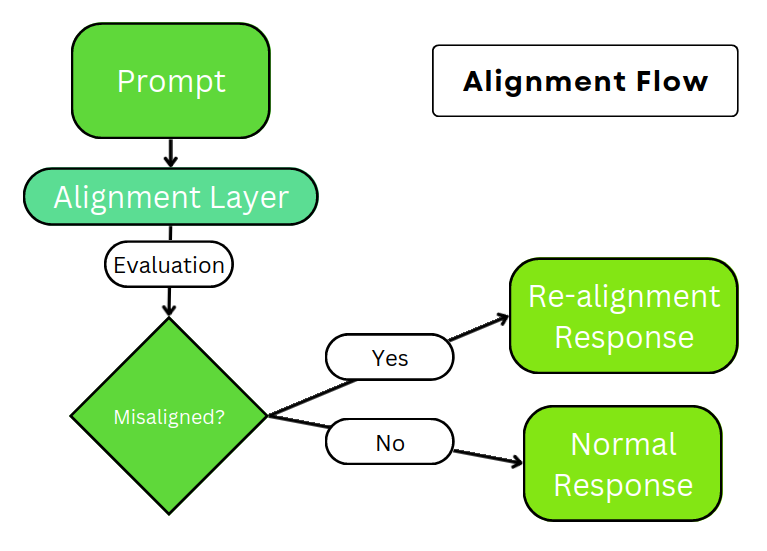
\includegraphics[width=\linewidth]{images/realignment}
            \caption{The \textit{Mathesis} Re-alignment Flow}\label{Fig:realignment}
        \end{minipage}\hfill
        \end{center}
    \end{figure}

    \section{Conclusion}

    \subsection{Future Work}
    In our future work in this project, we expect to both finalize the attributes of the project that
    we have included in its current scope and to expand the projects scope to cover more edge cases.

    We aim to better handle reasonable edge cases by assisting students with navigating the new system,
    managing adversarial attacks, and further automating the model training process on new datasets.
    These enhancements will help students adapt to the \textit{Mathesis} assistant and its learning platform,
    deter them from using the model for unintended purposes, and create a conducive environment for
    professors who wish to integrate their courses into the learning system in future semesters.

    A member of our team will continue to monitor and maintain the \textit{Mathesis} learning assistant as it
    is integrated into our pilot program in Introduction to Biology. This member will assist in user
    support and training during the semester and coordinate with the course’s faculty member to
    facilitate a seamless integration. During and after the conclusion of our pilot semester, we will
    generate metrics which assess the competency of students to achieve the course’s key learning
    objectives and compare with a control section of the course taught by the same faculty member.
    We hope these metrics, and the student and faculty feedback resulting from our pilot program will
    indicate to the RPI community that personalized AI tutors can be successful in promoting student
    engagement and comprehension.

    \subsection{Closing Thoughts}
    Our project has the potential to make a significant impact on higher education, specifically in
    facilitating personalized learning experiences for students. By providing a knowledgeable and
    adaptive AI learning assistant, we aim to promote active engagement, reduce stress, and ensure a
    transparent learning environment for both students and instructors.

    The success of \textit{Mathesis} in the Introduction to Biology course at RPI will serve as a
    stepping stone for its future integration into various other university courses. We believe that
    personalized AI tutors can be particularly beneficial in courses where providing individualized
    feedback to each student can be challenging due to high enrollment numbers or limited instructor
    resources.

    By aligning our project with the fourth UN SDG, we aim to contribute to the global goal of
    ensuring inclusive and equitable quality education and promoting lifelong learning opportunities for
    all. We envision \textit{Mathesis} becoming a scalable and adaptable platform that can be integrated
    into different educational frameworks, fostering a culture of continuous lifelong learning and improvement.

    \pagebreak
    
    \bibliographystyle{abbrv}
    \bibliography{references}

    \pagebreak

    \begin{appendices}

        \setcounter{section}{0}
        \section{Use Case Document}

        \begin{table}[H]
        \label{tab:useCaseDoc1}
        \centering
        \def\arraystretch{1.4}
        \begin{tabular}{|p{13cm}|}
            \hline
            \textbf{Use Case Name:} GPT Pedagogy: Mathesis\\\hline

            \textbf{Goal:}\\

            Develop a model, \textit{Mathesis}, that maintains its conversational abilities,
            while embedding additional knowledge about faculty defined key learning objectives.
            This model will generate a series of topic-relevant questions, evaluate the answers of
            those questions, and give useful feedback or counterexamples to the student.\\\hline

            \textbf{Summary:}\\

            Students can log in and can start chatting with our agent as it
            responds in real time with auto-generated responses. They can then proceed with their
            learning experience and discover gaps in their knowledge through their chat and through
            quizzes.  This leads to better overall learning outcomes.

            Faculty can log in and start viewing a summary of student responses to knowledge.
            Through this, they can pinpoint gaps in the collective student knowledge, drawing
            unbiased conclusions, and making necessary changes of pace for later lectures.  This then
            improves the quality and consistency of lectures, leading to a better teaching experience.
            \\\hline

            \textbf{Actors:}\\

            Students, Faculty, Server, \textit{Mathesis} model, Database\\\hline

            \textbf{Preconditions:} \\\makecell[l]{
                \tabitem The User has a valid RPI ID.
                \tabitem The User is enrolled in the class either as the professor or student.
                \tabitem The User is connected to the internet.
                \tabitem The Server is running.
                \tabitem OpenAI is accessible.
                \tabitem DataBase is accessible.
            }\\\hline

        \end{tabular}
        \end{table}

        \begin{table}[H]
        \label{tab:useCaseDoc2}
        \centering
        \def\arraystretch{1.4}
        \begin{tabular}{|p{13cm}|}
            \hline

            \textbf{Triggers:} \\\makecell[l]{
                \tabitem User sends a request to load the homepage.
                \tabitem User sends a chat request to the model.
                \tabitem User selects a lesson from the list.
                \tabitem User submits a quiz from a lesson.
                \tabitem Faculty user submits a request to generate a new question.
                \tabitem Faculty user saves a quiz configuration
                \tabitem Faculty requests student performance report.
            }\\\hline

            \textbf{Basic Flow:} \\\makecell[l]{
                \\1. The user logs in via their RPI account.
                \\2. Server checks if the information matches and if the user is
                    \\\quad~enrolled in the class or not.
                \\3. Server create response to the user.
                \\4. Users interprets the response and sends a request to the server.
                \\5. Server interprets the result and sends a request to OpenAI API.
                \\6. OpenAI sends the generated result back to the server.
                \\7. Server pushes the response back to the user and the database.
                \\8. User interprets the response.
                \\9. Database records the response and terminates the use case.
            }\\\hline

            \textbf{Alternate Flow:} \\\makecell[l]{
                \\1. A faculty user logs in via their RPI account.
                \\2. Server checks if the information matches and if the faculty is
                    \\\quad~enrolled in the class or not.
                \\3. Faculty member requests the generation of a new question for a
                    \\\quad~lesson quiz.
                \\4. \textit{Mathesis} generates the selected question and it is returned
                    \\\quad~to the UI.
                \\5. Faculty member removes quiz questions, inserts generated qustions,
                    \\\quad~or both.
                \\6. Faculty saves the lesson quiz to the database.
                \\7. Database records the new quiz and terminates the use case.
            }\\\hline

            \textbf{Exception Flow:} \\\makecell[l]{
                \\1. The user logs in via their RPI account.
                \\2. Server checks if the information matches and if the user is
                    \\\quad~enrolled in the class or not.
                \\3. User performs actions beyond the normal usage of \textit{Mathesis}.
                \\4. \textit{Mathesis} detects malicious behavior.
                \\5. User interaction redirected and actions are taken to either mitigate
                    \\\quad~or terminate this incident.
            }\\\hline

        \end{tabular}
        \end{table}

        \begin{table}[H]
        \label{tab:useCaseDoc3}
        \centering
        \def\arraystretch{1.4}
        \begin{tabular}{|p{13cm}|}
            \hline

            \textbf{Postconditions:} \\\makecell[l]{
                \tabitem Students have gained further course knowledge.
                \tabitem Students have their knowledge tested with results recorded.
                \tabitem Faculty has observed student performance.
                \tabitem Faculty has modified lessons to account for students' knowledge.
            }\\\hline

            \textbf{Activity Diagram:}\\

            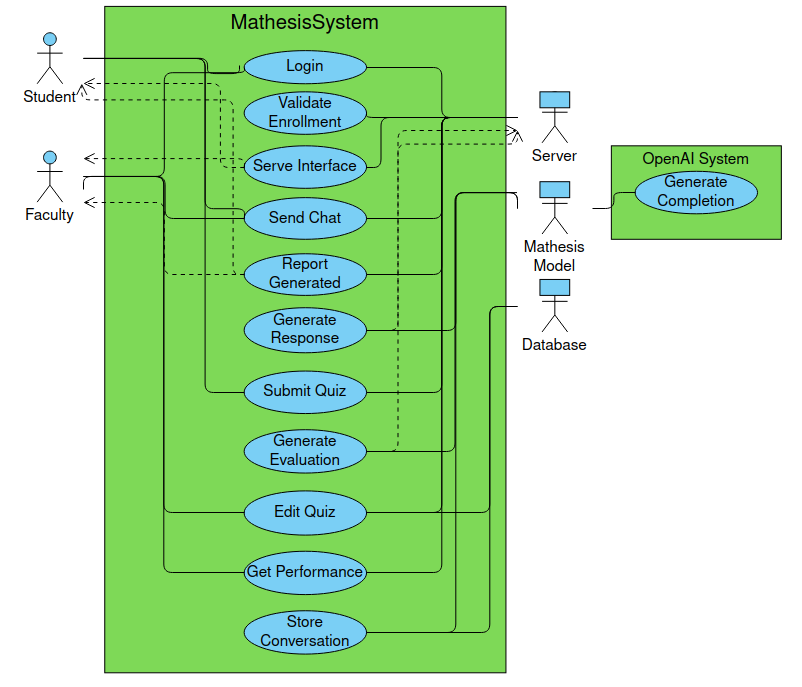
\includegraphics[width=\linewidth]{images/newActivityDiagram}\\\hline

            \textbf{Questions and Answers:} \\\makecell[l]{
                \tabitem What role does the success of \textit{Intro to Biology} trial play in this
                    \\\quad~use case?\\
                    \\\quad~The success of Mathesis in the \textit{Introduction to Biology}
                    \\\quad~course at RPI will serve as a stepping stone for its future
                    \\\quad~integration into various other university courses.\\
                \tabitem How can faculty/professors draw conclusions from student responses?\\
                    \\\quad~The student feedback report will contain important information
                    \\\quad~about which students struggle the most on certain topics
                    \\\quad~along with the areas that the class as a whole is the least
                    \\\quad~knowledgeable in.  This will hopefully help faculty to decide
                    \\\quad~how to best allocate their time during course lectures or assignments.
            }\\\hline
        \end{tabular}
        \end{table}

    \end{appendices}
\end{document}
